% TODO:
% - Make a tool for download and transformation of datasets, and sell the work that I have done
% - Compare single user datasets
% - group rec datasets mention
% - do dataset group augmentation and add it to the tool


\chapter{Datasets}  \label{chap:datasets}
People are gregarious in nature, but the same, unfortunately, cannot be said about machine learning datasets. Vast majority of them are not directly usable in the group RS research due to only containing information about single user preference. In order to design and evaluate group recommender systems, we preferably need datasets that contain information about groups' preference.

In this chapter, we will start with description of which datasets are suitable for the use in RS domain. We describe commonly used datasets in the non-group RS domain. Analyse their high level properties and describe what transformations are needed in order to make the use of the dataset convenient. 

Next, we will talk about the existing group RS datasets and introduce methods that can be used to generate the group recommendation information synthetically from non-group RS datasets. We will use these methods to generate standardized synthetically enriched group RS datasets from non-group datasets that we will describe in the single user datasets subchapter.

And finally, we will describe a data transformation library that we have created for the purpose of simplifying the research efforts in the RS domain and for evaluation of our proposed algorithm.

% We will first describe a few of the popular datasets which we have determined to be used as research data the most. Then we will 

% -------------------------------------------------------------------------------------
\section{Single user datasets}
% -------------------------------------------------------------------------------------
Multiple well known and thoroughly studied datasets exist in the recommender system domain. Let us now present the popular ones that seems to be utilized the most.

If we talk about specific format of the data then we are referring to the unified format into which we have transformed the original data into using the dataset transformation library. Further description about the data format transformations follow in \ref{subsec:04_single_user_datasets.gathering_processing}.



% -------------------------------------------------------------------------------------
\subsection{Movie Lens}
% -------------------------------------------------------------------------------------
One of the most well known dataset in the RS domain, it contains 25 million ratings in total across 62,000 movies and 162,000 users. The data were collected between 1995 and 2019 and the current version of this size (25M) was released in November of 2019. Data are organic and come from a web-based recommendation system at \href{https://movielens.org/}{movielens.org}. The project was specifically created in order to gather research data on personalized recommendation by researches at University of Minnesota.

Dataset is in a good format that is quite easy to parse and use. Further description follows in \ref{subsec:04_single_user_datasets.gathering_processing}.

\hfill \break
\noindent
\textbf{Number of items:} 62,000 \newline
\textbf{Number of users:} 162,000 \newline
\textbf{Number of user-item interactions:} 25,000,095 \newline
\textbf{User-item interactions format:} Sparse matrix of ordinal ratings [1, 1.5, 2, ... 4.5, 5] - user rated a movie \newline
\textbf{List of datatables:} Movies (detail in table \ref{table:5.1_ML_movies}), Ratings (detail in table \ref{table:5.1_ML_ratings}), Tags, Links, Genres, Genome Scores, Genome Tags

\begin{table}[!ht]
\centering
\begin{tabular}{ l l }
\verb|item_id| & \verb|title| \\
    \hline
     1  &                   Toy Story (1995) \\
     2  &                     Jumanji (1995) \\
     3  &            Grumpier Old Men (1995) \\
   ...  &                                ... \\
209169  &                A Girl Thing (2001) \\
209171  &     Women of Devil's Island (1962) \\ [1mm]
\multicolumn{2}{l}{{[62423 rows x 2 columns]}}
\end{tabular}
\caption{Short snippet of Movie Lens dataset's \texttt{movies.csv} table.}
\label{table:5.1_ML_movies}
\end{table}

\begin{table}[!ht]
\centering
\begin{tabular}{ l l l l }

% \texttt{user\_id} & \texttt{item\_id} & \texttt{rating} & \texttt{timestamp} \\
\verb|user_id| & \verb|item_id| & \verb|rating| & \verb|timestamp| \\
    \hline
    1 &      296  &   5.0 & 1147880044 \\
    1 &      306  &   3.5 & 1147868817 \\
    1 &      307  &   5.0 & 1147868828 \\
  ... &      ...  &   ... &        ... \\
162541 &    58559  &   4.0 & 1240953434 \\
162541 &    63876  &   5.0 & 1240952515 \\ [1mm]
\multicolumn{4}{l}{{[25000095 rows x 4 columns]}}
\end{tabular}
\caption{Short snippet of Movie Lens dataset's \texttt{ratings.csv} table.}
\label{table:5.1_ML_ratings}
\end{table}

% This dateset contains information about movies in the form of \textit{'\textless movieId, title, genres\textgreater'}, ratings in the form of \textit{'\textless userId, movieId, rating, timestamp\textgreater'} and additional information about links, tags, genome-scores and genome-tags.




% -------------------------------------------------------------------------------------
\subsection{KGRec}
\label{subsec:04_single_user_datasets.kgrec}
% -------------------------------------------------------------------------------------
KGRec is a smaller and less known dataset. We have chosen this dataset due to it being utilized in GFAR method introduced in \cite{GFAR-kaya2020} and described in \ref{subsec:03_advanced_methods.gfar}. This dataset consists of two separate datasets of music and sound, KGRec-music and KGRec-sound respectively.

The first music dataset comes from \href{https://www.songfacts.com/}{songfacts.com} (items and text descriptions) and \href{https://www.last.fm/}{last.fm} (ratings, items, tags). Each user-item interaction is a user listening to a song.

The second, sound dataset, comes from \href{https://freesound.org/}{freesound.org}. Items are sounds with description using text and tags that were created by the person that uploaded the sound. Each user-item interaction is a user downloading an item, in this case a sound.

Further, we will consider only the music dataset and not utilize the sound dataset at all. We have made this decision to simplify comparisons and due to the origin of the sound dataset itself. It comes from a web-page where users can upload and download random sounds of their choosing, such as 'Mechanical clock movement' sound, 'Industrial elevator' sound and so on. The need for these sounds are most probably driven from people that are using them for their profession, such as video production and therefore does not reflect natural content consumption preferences.

Both datasets were created for the needs of \cite{kgrec_dataset_origin}, where they were introduced, they are altered for the needs of research in Recommendation Knowledge Graphs. Further, the original data that were used for creation of this datasets are described in \cite{kgrec_dataset_origin_full}.


\hfill \break
\noindent
\textbf{Number of items:} 8,640; 21,552\footnote{Number of items, users and user-item interactions are in order - music dataset; sound dataset} \newline
\textbf{Number of users:} 5,199; 20,000 \newline
\textbf{Number of user-item interactions:} 751,531; 2,117,698 \newline
\textbf{User-item interactions format:} one-valued implicit feedback - user listened or downloaded a song/sound \newline
\textbf{List of datatables:} Ratings(detail similar to \ref{table:5.1_KGRec_ratings}), Tags, Descriptions

\begin{table}[!ht]
    \centering
    \begin{tabular}{ l l }
        \verb|user_id|   & \verb|item_id| \\
        \hline
        7596     &  68  \\
        7596     & 130  \\
        7596     & 330  \\
        ...      & ...  \\
        50572897 & 8618 \\
        50572897 & 8619 \\ [1mm]
        \multicolumn{2}{l}{{[751531 rows x 2 columns]}}
    \end{tabular}
    \caption{Short snippet of KGRec dataset's \texttt{music\_ratings.csv} table.}
    \label{table:5.1_KGRec_ratings}
\end{table}

% \newline
% Both dataset are in the form of '\textlessuser userId, itemId\textgreater'


% -------------------------------------------------------------------------------------
\subsection{Netflix Prize}
% -------------------------------------------------------------------------------------

Data that were originally released in 2009 by the Netflix.com video streaming company for the \textit{Netflix Prize}, open competition with main prize of 1 million dollars. It contains data of more than 400 thousand randomly selected users from the company's database. Data contain information about users ratings of movies. It was originally available on the contest web page, but has been removed since.

The original data was split into multiple files in a file for ratings per movie manner. Each rating is a quadruplet of the form '\textless user, movie, date of rating, rating\textgreater'.

\hfill \break
\noindent
\textbf{Number of items:} 17,770 \newline
\textbf{Number of users:} 480,189 \newline
\textbf{Number of user-item interactions:} 100,480,507 \newline
\textbf{User-item interactions format:} sparse matrix of ordinal ratings [1, 2, 3, 4, 5] \newline
\textbf{List of datatables:} Ratings (detail in table \ref{table:5.1_Netflix_ratings}), Movies (detail in table \ref{table:5.1_Netflix_movies})

\begin{table}[!ht]
    \centering
    \begin{tabular}{ l l l l }
        \verb|user_id| & \verb|item_id| & \verb|rating| & \verb|date| \\
        \hline
              6 &             30 &             3 &  2004-09-15 \\
              6 &            157 &             3 &  2004-09-15 \\
              6 &            173 &             4 &  2004-09-15 \\
            ... &            ... &           ... &         ... \\
        2649429 &          17627 &             3 &  2003-07-21 \\
        2649429 &          17692 &             2 &  2002-12-07 \\ [1mm]
        \multicolumn{4}{l}{{[100480507 rows x 4 columns]}}
    \end{tabular}
    \caption{Short snippet of Netflix dataset's \texttt{ratings.csv} table.}
    \label{table:5.1_Netflix_ratings}
\end{table}
    
\begin{table}[!ht]
    \centering
    \begin{tabular}{ l l l }
        \verb|item_id| & \verb|release_year| & \verb|title| \\
        \hline
            1 &       2003.0 &            Dinosaur Planet    \\
            2 &       2004.0 & Isle of Man TT 2004 Review    \\
            3 &       1997.0 &                  Character    \\
          ... &          ... &                        ...    \\
        17769 &       2003.0 &                The Company    \\
        17770 &       2003.0 &               Alien Hunter \\ [1mm]
        \multicolumn{3}{l}{{[17770 rows x 3 columns]}}
    \end{tabular}
    \caption{Short snippet of Netflix dataset's \texttt{movies.csv} table.}
    \label{table:5.1_Netflix_movies}
\end{table}
% -------------------------------------------------------------------------------------
\subsection{Spotify - Million Playlist Dataset}
% -------------------------------------------------------------------------------------
This dataset was released in January 2018 for \textit{The Spotify Milion Playlist Dataset Challenge}. It contains 1,000,000 playlists with information about tracks that are part of each playlist. Main purpose of this dataset was to study and develop better algorithms for automatic playlist continuation where the system would be able to recommend songs that are similar to those that are already in the playlist. In contrast to the Netflix challenge, no prize was to be awarded at the end of the challenge.

Even though the context of this dataset are playlists and not users, we propose a different view on the dataset, where each playlist will represent a single user. This way, we have an another big and organic dataset at our disposal. It can therefore be used not only for playlist continuation tasks, but for the classical RS domain tasks as well. In a sense, a single playlist is a specific subset of preference of the user that have created the playlist. Therefore we expect to see a narrower preference distribution for each of these 'playlist' users.

For completeness, it is necessary to add that some playlists are 'collaborative', meaning that they were created by multiple users. But they account for only 2.3\% of all playlists, which in our opinion does not substantially affect the dataset. These collaborative datasets could be used as a group recommender dataset on their own, unfortunately, the information about which user added which track, to the collaborative playlist, is not present.

\begin{table}[!ht]
    \centering
    \begin{tabular}{ l l }
        \verb|playlist_id|   & \verb|item_id| \\
        \hline
        549000     &  0  \\
        549000     & 1  \\
        549000     & 2  \\
        ...      & ...  \\
        302999 & 133087 \\
        302999 & 133088 \\ [1mm]
        \multicolumn{2}{l}{{[66346428 rows x 2 columns]}}
    \end{tabular}
    \caption{Short snippet of Spotify Milion Playlist dataset's \texttt{ratings.csv} table.}
    \label{table:5.1_Spotify_ratings}
\end{table}


\begin{table}[!ht]
    \centering
    \begin{tabular}{ l l l }
        \verb|item_id| & \verb|item_name| & \verb|artist_name|  \\
        \hline
             0 & Boots of Spanish Leather &         Bob Dylan \\
             1 &       Mr. Tambourine Man &         Bob Dylan \\
             2 &             Danny's Song & Loggins \& Messina \\ 
           ... &                      ... &               ... \\
       2262290 &               Robin Hood &        Crazy Fool \\
       2262291 &                Guilttrip &      Ace Reporter \\ [1mm]
       \multicolumn{3}{l}{{[2262292 rows x 6 columns]}}
    \end{tabular}
    \caption[Short snippet of Netflix dataset's \texttt{tracks.csv} table.]{Short snippet of Netflix dataset's \texttt{tracks.csv} table. (Columns \texttt{item\_uri}, \texttt{artist\_uri}, \texttt{album\_uri}, containing URI to Spotify object were omitted for simplicity due to their substantial length.)}
    \label{table:5.1_Spotify_tracks}
\end{table}

\hfill \break
\noindent
\textbf{Number of items:} 2,262,292 \newline
\textbf{Number of users:} 1,000,000 \newline
\textbf{Number of user-item interactions:} 66,346,428 \newline
\textbf{User-item interactions format:} one-valued implicit feedback - user added a song to a playlist\newline
\textbf{List of datatables:} Tracks (detail in table \ref{table:5.1_Spotify_tracks}), Ratings (detail in table \ref{table:5.1_Spotify_ratings})




% -------------------------------------------------------------------------------------
\subsection{Comparison of datasets}
% -------------------------------------------------------------------------------------

\begin{figure}[ht!]
    \centering
    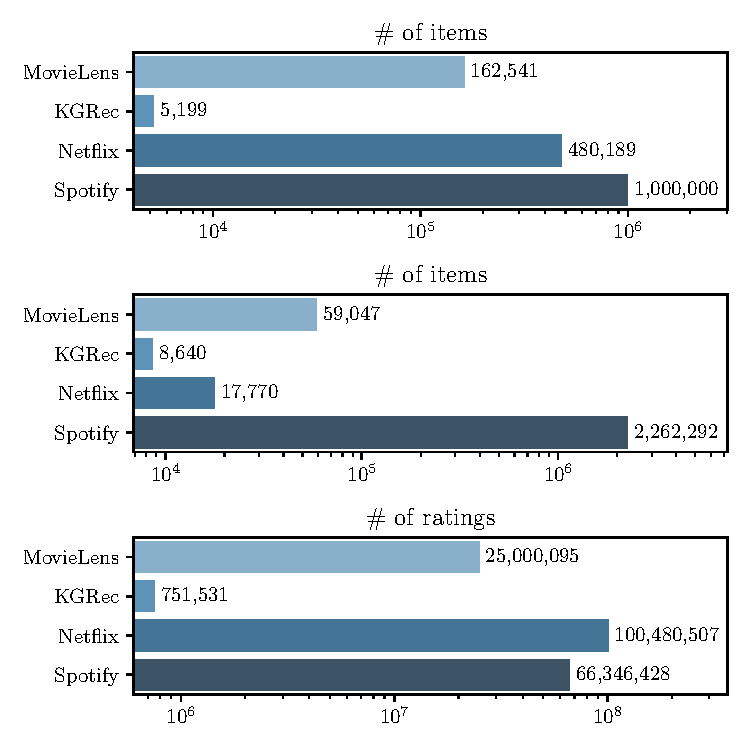
\includegraphics{img/figures/datasets_counts.pdf}
    \caption[Size comparison of the selected datasets.]{Size comparison of the selected datasets. All x-axes are log scale due to the big differences between the dataset.}
    \label{fig:datasets_counts}
\end{figure}

We have described each dataset separately, let us now compare them together to see how they differ. As we can see on \ref{fig:datasets_counts} the Spotify and Netflix datasets are the biggest. We see that KGRec dataset is almost two orders of magnitude smaller than the rest of the datasets. As already mentioned, we have selected it due to it being utilized in the related literature, mainly in \cite{GFAR-kaya2020} as mentioned in \ref{subsec:03_advanced_methods.gfar}. Spotify dataset is different by having two orders of magnitude more items, which can present a challenge on its own. If we for example use matrix factorization methods to compute the preference, then the amount of memory will rise by two orders of magnitude as well. Additionally, the sparsity of ratings is higher, which can negatively affect efficacy.

Movie Lens dataset has a potential benefit as it has actual ratings for each user-item interaction. All other presented datasets only contain user-item interactions in the form of one-valued implicit feedback, where Spotify has the item-playlist interaction instead of user-item interaction.

\begin{figure}[ht!]
    \centering
    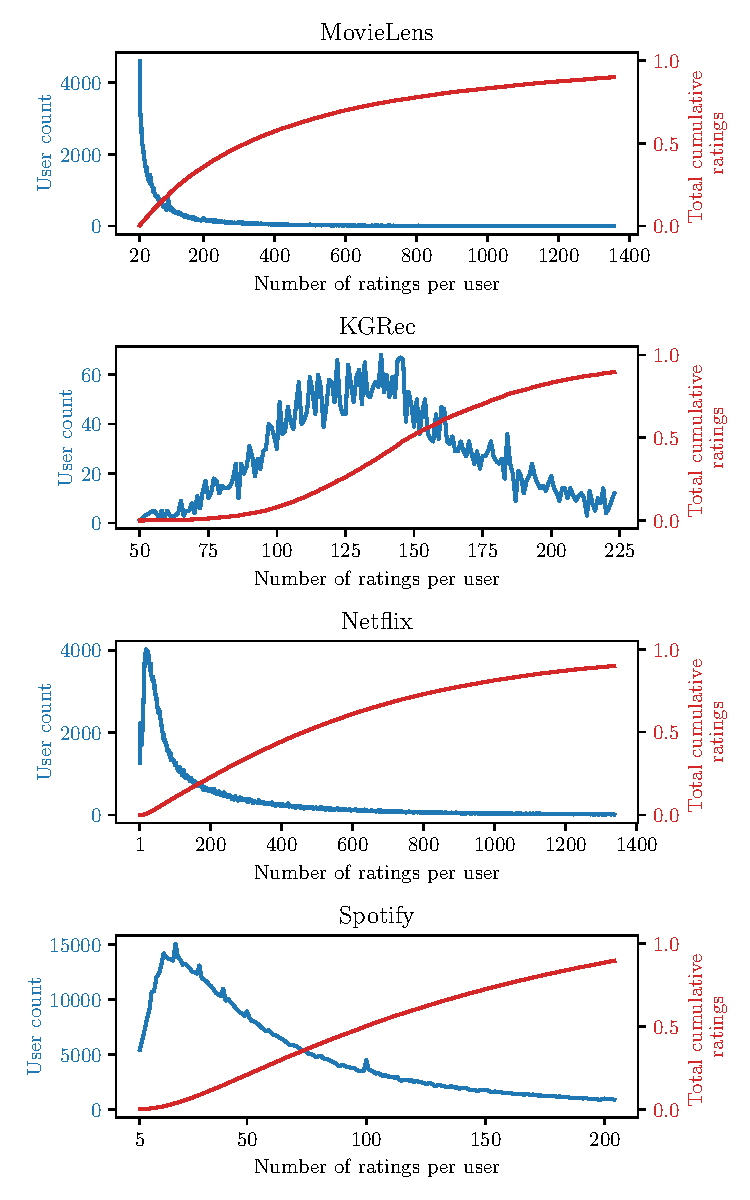
\includegraphics{img/figures/num_users_by_rating_count.pdf}
    \caption[Distribution of ratings]{Distribution of ratings for groups of users by how many ratings they have made. Blue line shows how many users have made that particular amount of ratings, while red line shows the total cumulative mass distribution of ratings. We have clipped the number of ratings by total cumulative ratings of 90\% due to very long-tailed data, where some small amount of users created a very high amount of ratings.}
    \label{fig:datasets_num_ratings}
\end{figure}

On \ref{fig:datasets_num_ratings} we present the distribution of ratings among users. The left y-axis, blue, present user count of users with particular number of ratings. We have clipped the users with high number of ratings so that we can better see the interesting part of the data, which would otherwise be squashed by the long tails. The clip was made on the last 10\% mass of all ratings.

We see, that Movie Lens has the most natural ratings distribution. In this dataset, only users with more than 20 ratings are present which is visible on the figure as well and it is most probably the reason why we do not see the same initial rise in ratings as for Netflix and Spotify datasets''

KGRec dataset is different, it is more jagged due to smaller effect of being smoothed out by the the amount of data as with the other datasets. Interestingly enough, by contrast to the other datasets the number of users does not follow an exponential distribution. At first, we thought that the reason for it is, that the dataset was gathered at a website where users listen and download songs that are always a part of an album and therefore always downloading many songs at once, but that would not explain why this rise starts at number of ratings around 75.

The true reason for this can be partially found in the original paper - \cite{kgrec_dataset_origin}. As already described in \ref{subsec:04_single_user_datasets.kgrec} the dataset was altered to better fit the required research objective of recommendation using knowledge graphs. Where songs with less than 10 interactions are removed, users with less than 50 item interactions are removed and only songs with over average plays are counted as a user-item interaction. But this would not explain the non exponential nature of the distribution. We have downloaded and explored the original dataset from \cite{kgrec_dataset_origin_full}, the original dataset is not only a one-valued implicit feedback but it is the number of times a user has played the song. When we visualise the original dataset using 'sum of plays per user' instead of 'count of interactions per user', then we get a natural looking exponential distribution. Therefore, the most probable reason for the KGRec's dataset distribution is that users like to replay a smaller amount of songs multiple times which then creates more of a normal looking distribution.

Further, Netflix dataset look similar to Movie Lens with two exceptions. First being that Movie Lens includes only users with at least 20 ratings, therefore the initial increase in number of ratings is not visible. Secondly, both Netflix and Spotify datasets have cumulative rating distribution shifted more to the right, which means that there is more ratings among users that were more active on the service and have more ratings.




% -------------------------------------------------------------------------------------
\subsection{Datasets gathering and processing} \label{subsec:04_single_user_datasets.gathering_processing}
% -------------------------------------------------------------------------------------

Processing the above mentioned datasets was more difficult than it should have been. They are not easily accessible, some of them are available only behind a login wall and in different, incompatible and non standard formats. We have therefore processed and unified these datasets using a tool that we have developed. At first, we wanted to have a shared storage where they would be available in already transformed form, but that is not feasible due to datasets' licences. Let us now describe data transformations that we have done for each of the datasets. We aim to have the datasets in standard zipped CSV format that can be easily loaded by most of the popular data manipulation tools such as Pandas. Additionally, if not misleading, we prefer the columns of the datasets to be named in unified fashion.

\begin{itemize}
    \item \textbf{Movie Lens} dataset is available at the the authors web page \newline \href{https://grouplens.org/datasets/movielens/25m/}{grouplens.org/datasets/movielens/25m/}. It is easily accessible and ready-to-be-used dataset (files in valid CSV format, zipped together in a single archive). This was the nicest dataset to start working with. No transformations were necessary.
    
    \item \textbf{KGRec} dataset is available for download at the authors web page\newline \href{https://www.upf.edu/web/mtg/kgrec}{upf.edu/web/mtg/kgrec}. Unfortunately, downloading the dataset is not straightforward due to the download link being an unsecured http on a secured https site. This is a problem while using modern browsers which do not support mixed http and https content. The dataset has ratings in a standard CSV form with redundant information about the incidence, which is always of value 1. Main data in sparse incidence matrix representation are in the form of '\textless userId, itemId\textgreater'. Additional data with tags and descriptions of items are separated into individual files in the original dataset, we have transformed them into two CSV tables of form '\textless itemId, tags\textgreater' and '\textless movieId, description\textgreater' respectively.
    
    \item \textbf{Netflix} dataset is available at an independent web page
    \newline
    \href{https://www.kaggle.com/datasets/netflix-inc/netflix-prize-data}{kaggle.com/datasets/netflix-inc/netflix-prize-data}.
    The original web page of the challenge is no longer available. The dataset was additionally processed by the uploader by aggregating the small per movie rating files into four bigger files. This dataset was in non-standard format where ratings were not in CSV but in a custom format reflecting the original movie ratings per file division. Each group of ratings for a movie starts with a line only containing the id of the movie and a colon, then ratings for the movie follow each per line in a format '\textless user-id,rating,timestamp\textgreater'.
    
    \item \textbf{Spotify} dataset is available at AIcrowd.com where the original Spotify challenge was introduced. Unfortunately, the dataset is behind a login wall. After registering and logging in, it can be downloaded from \newline\href{https://www.aicrowd.com/challenges/spotify-million-playlist-dataset-challenge}{aicrowd.com/challenges/spotify-million-playlist-dataset-challenge}.
    \newline
    
    The dataset is comprised of 1000 json files each describing 1000 playlists. The dataset contains a lot of information about each playlist such as the name, when it was modified, how many followers it has and so on. We go through all data and simultaneously create list of playlists to track mapping and another list with any additional track information, such as the Spotify URI links for the track, album and artist. We have created a separate numerical track id due to the native one of track URI being too long. Apart from the json files, the zip archive contains some python code to provide easy parsing and simple statistics about the dataset.
    
\end{itemize}


% todo: pocet ratingu
% srovnat itemy podle toho kolik lidi hodnotilo a zobrazit prumerny rating





A simple python snippet is provided that can be used to easily download the available datasets.


% -------------------------------------------------------------------------------------
\section{Group datasets}
% -------------------------------------------------------------------------------------
Let us now investigate datasets that contain information about groups of users. We will look through some of the datasets mentioned in related literature in the group recommender system domain.

\subsection{Datasets overview}\label{subsection:04_}

When reading through related literature on the topic of GRS, we have mostly encountered synthetically created datasets either from the Movie Lens dataset or from the Netflix dataset. The main reason for not utilizing datasets that have innate group information is that there is not many of them. Let us now go through some of the mentioned datasets from the related literature and determine their suitability for the use in group recommender system research.

First, we would like to point out, that most papers in our domain that do not use the more traditional Movie Lens or Netflix datasets and instead use less known datasets. That would be an entirely valid thing to do if there is not a total lack of description about where and how the dataset can be obtained and or how the raw dataset was filtered and altered. Most papers only mention which dataset they were using and some high level information about the dataset such as number of users, items and interactions. This makes the papers' experiments irreproducible and unverifiable. Same can sometimes be said about papers that use single user datasets with synthetically generated group information. Some of the time, it is not entirely clear as of how the synthetic groups were generated or how were parameters of the synthetic group info creation set.

We have put together high level information about the some of the datasets in \ref{table:5.2_GRS_datasets_comparation}.

\begin{table}[!ht]
    \centering
    \begin{tabular}{ r | c c c c }
         & \#users & \#items & \#groups & avg. g. size \\
        \hline
            CAMRa2011\cite{attentative_group_recommendation}
                & 602 & 7,710 & 290 & ? \\
            Douban\cite{gowalla_weeplaces_yelp}
                & 23,032 & 10,039 & 58,983 & 4.2 \\
            Gowalla\cite{gowalla_weeplaces_yelp}
                & 25,405 &  38,306 & 44,565 &  2.8 \\
            Mafengwo\cite{attentative_group_recommendation}
                & 5,275 & 1,513 & 995 & ? \\
            Meetup\cite{meetup_origin}
                & 42,747 & 2,705 & 13,390 & 16.66 \\
            Plancast\cite{meetup_plancast}
                & 41,065 & 13,514 & 25,447 & 12.01 \\
            Yelp\cite{gowalla_weeplaces_yelp}
                & 7,037 & 7,671 & 10,214 & 6.8 \\
            Weeplaces\cite{gowalla_weeplaces_yelp}
                &  8,643 & 25,081 & 22,733 & 2.9 \\
    \end{tabular}
    \caption[Size overview of selected GRS datasets]{Size overview of selected GRS datasets. Note: Some dataset sizes are given after transforming the original datasets by removing users and items that are not part of any group.}
    \label{table:5.2_GRS_datasets_comparation}
\end{table}


\subsubsection{CAMRa2011} \label{subsubsec:04_group_datasets.overview.camra}
CAMRa2011 dataset was released in 2011 for 2011 ACM Recommender Systems Conference. The dataset is unavailable at the original location and we were unable to retrieve it from the web. Numbers in table \ref{table:5.2_GRS_datasets_comparation} are taken from \cite{attentative_group_recommendation}. We have found altered version of the dataset at \href{https://github.com/LianHaiMiao/Attentive-Group-Recommendation}{github.com/LianHaiMiao/Attentive-Group-Recommendation}, which is a GitHub repository for the code and experiments from \cite{attentative_group_recommendation}. The dataset is quite small and we are doubtful about its quality and source.


\subsubsection{Douban} \label{subsubsec:04_group_datasets.overview.douban}
This dataset has similar problems as the CAMRa2011 dataset, we are unable to retrieve it from the web. At the same time, in the already mentioned repository for \cite{attentative_group_recommendation}, we found an author's comment about adding the dataset soon (in 2018), which was never done.


\subsubsection{Gowalla} \label{subsubsec:04_group_datasets.overview.gowalla}
Gowalla was a location based social network. It has been dissolved in 2012 when it was acquired by Facebook. The dataset contains people logging in locations that they have visited. The dataset can be easily downloaded at \href{https://www.yongliu.org/datasets/}{yongliu.org/datasets/}, we have discovered this page and dataset in \cite{gowalla_weeplaces_yelp}.

This dataset does not directly contain any group information but it could be inferred by combining the check-in data in of format '\textless userid, placeid, datetime\textgreater' and friendship data that link pairs of users '\textless userid1, userid2\textgreater'. If you and some of your friends visit the same place at around the same time, we can state that probably you were part of the same group. And if you visit more places together then the chance of a random occurrence drops significantly.

We suspect that due to the data being location based there will be a substantial location similarity bias where if you visit a certain place then you are very likely to visit a popular place nearby regardless of its quality.

\begin{itemize}
    \item \textbf{Available group information:} none explicit, can be interpolated from friendship information and user-item interaction timestamps
    \item \textbf{User-item interactions:} one-valued implicit feedback
    \item \textbf{Group-item interactions:} none
    \item \textbf{Items type:} Places check-ins
\end{itemize}


\subsubsection{Mafengwo} \label{subsubsec:04_group_datasets.overview.mafengwo}
Very small, proprietary dataset mentioned in paper  \cite{attentative_group_recommendation}. Dataset is unavailable for download. We were unable to find other source from where we would be able to download this dataset.


\subsubsection{Meetup} \label{subsubsec:04_group_datasets.overview.meetup}
This dataset is crawled data from website \href{https://www.meetup.com}{meetup.com} from \cite{meetup_origin} used in \cite{meetup_plancast}. Meetup is a popular web page for meeting other people with same hobbies and interests. This dataset contains only data from two regions, New York City and state of California. One substantial distinction from other datasets is that the items represent social events that a person can attend which happen only once. And are not repeating, this creates difficulties with similarity calculation between users.

With some difficulties we have downloaded the dataset from
\newline\href{https://personal.ntu.edu.sg/gaocong/datacode.htm}{personal.ntu.edu.sg/gaocong/datacode.htm}.

\begin{itemize}
    \item \textbf{Available group information:} group memberships, groups are on average big
    \item \textbf{User-item interactions:} one-valued implicit feedback
    \item \textbf{Group-item interactions:} none
    \item \textbf{Items type:} Social events
\end{itemize}


\subsubsection{Plancast} \label{subsubsec:04_group_datasets.overview.plancast}
Unfortunately we were unable to obtain this dataset for further analysis. In \cite{meetup_plancast} where this dataset is mentioned, there is no download link, only a reference to \cite{plancast_origin} where no additional information about the source is provided.

\subsubsection{Yelp}\label{subsubsec:04_group_datasets.overview.yelp}
This dataset contains reviews for businesses and places. In \cite{gowalla_weeplaces_yelp} they use a subset of the whole dataset only for the city of Los Angeles, the whole dataset can be downloaded at \href{https://www.yelp.com/dataset}{yelp.com/dataset} and in its unfiltered variant is vastly bigger than other mentioned datasets with over 6,9 million ratings.

\begin{itemize}
    \item \textbf{Available group information:} none explicit, can be interpolated from friendship information and user-item interaction timestamps
    \item \textbf{User-item interactions:} one-valued implicit feedback and text reviews
    \item \textbf{Group-item interactions:} none
    \item \textbf{Items type:} Places check-ins
\end{itemize}


\subsubsection{Weeplaces} \label{subsubsec:04_group_datasets.overview.weeplaces}
Similarly to Gowalla dataset, Weeplaces was a website that aimed to visualize users' location based check-in activities. It has been integrated with multiple location-based social networking services such as Foursquare or Facebook.
It contains information about check-ins and friendships, same as the Gowalla dataset. It can be downloaded from \href{https://www.yongliu.org/datasets/}{yongliu.org/datasets/}. We have discovered this page and dataset in \cite{gowalla_weeplaces_yelp}.
Same arguments for the group information and location based bias hold for this dataset, again, same as for Gowalla dataset. 

How are groups created is not described in the original paper. Other information which is missing is a full description of how was the raw dataset transformed and filtered. High level description is present, but it is incomplete.


\begin{itemize}
    \item \textbf{Available group information:} none explicit, can be interpolated from friendship information and user-item interaction timestamps
    \item \textbf{User-item interactions:} one-valued implicit feedback
    \item \textbf{Group-item interactions:} none
    \item \textbf{Items type:} Places check-ins
\end{itemize}


\subsubsection{Dataset selection}
Let us now select subset of the mentioned datasets for further analysis and for inclusion to our download and transform tool.

We have rated all datasets on a scale of 'poor', 'ok' and 'good' in \ref{table:5.2_GRS_datasets_rating} for the following important criteria:
\begin{itemize}
    \item \textbf{Ease of retrieval} \newline
        We award 'poor' rating if the dataset cannot be downloaded at all. 'ok' rating if we can download the dataset with some difficulties from either the source in the mentioned paper or any of the related linked papers, we well as if we can download the dataset from an unrelated source. We award 'good' rating if the dataset is easily downloadable using the original sources or any source original to the dataset, such as the original research challenge web page.
    \item \textbf{Available group information} \newline
        We award 'poor' rating if the group information is either not very fitting to our use case, if the dataset does not contain any, or the group information is very scarce. We award 'ok' and 'good' in cases where the information is present and the the quality is good or great respectively. Ideal situation is if the dataset contains a full information about which members were part of the group-item interaction and when the group-item interaction is rated by each member.
    \item \textbf{Size}\newline
        We award 'poor' if the dataset size is borderline unusable (the definition of what size is and isn't usable can differ widely based on the utilized methods). We award good, if the amount of information is on the order of information we can find in single user datasets. We award 'ok' to sizes in between.
    \item \textbf{Source legitimacy} \newline
        We award 'poor' if the dataset comes from either not well known service of from a service that is already canceled. We award 'ok' if the source is less well known but legitimate and easily traceable and finally we award 'good' if the source is a well known service used around the world.
\end{itemize}

Additionally, some criteria that we were unable to assess (due to the dataset not being available for download) were marked 'n/a'.

With all relevant information about each dataset that can be found in the current subchapter and in \ref{table:5.2_GRS_datasets_rating}, we have chosen datasets that do not have the rating 'poor' in any of the mentioned criteria. %The only datasets that fulfill these criteria are Yelp and Weeplaces datasets. We will include them in our dataset comparison and add to our Dataset downloader tool.

Unfortunately no datasets that we have explored currently satisfy our criteria. Gowalla, Weeplaces and Yelp datasets are borderline usable with retrieving the group information from friendships and timestamps of reviews. But then belonging to a group requires us to set a window parameter, either floating or fix. Further Meetup dataset can be used, but with this dataset the average group size is unnaturally high, especially for researching fairness which in the context of big groups of unrelated people stops being relevant.

\begin{table}[!ht]
    \centering
    \begin{tabular}{ r | c c c c | c}
         & \makecell[c]{ease of \\ retrieval} & \makecell[c]{available \\ group \\ information} & size & \makecell[c]{source \\ legitimacy} & selected\\
        \hline
            % CAMRa2011
            \nameref{subsubsec:04_group_datasets.overview.camra}
                & poor & n/a & poor & poor & no\\
            % Douban
            \nameref{subsubsec:04_group_datasets.overview.douban}
                & poor & n/a & ok & poor & no \\
            % Gowalla
            \nameref{subsubsec:04_group_datasets.overview.gowalla}
                & good & poor & ok &  ok & no\\
            % Mafengwo
            \nameref{subsubsec:04_group_datasets.overview.mafengwo}
                & poor & n/a & poor & poor & no\\
            % Meetup
            \nameref{subsubsec:04_group_datasets.overview.meetup}
                & ok & poor & ok & good & no\\
            % Plancast
            \nameref{subsubsec:04_group_datasets.overview.plancast}
                & poor & n/a & ok & poor & no\\
            % Yelp
            \nameref{subsubsec:04_group_datasets.overview.yelp}
                & good & poor & ok & good & no\\
            % Weeplaces
            \nameref{subsubsec:04_group_datasets.overview.weeplaces}
                &  good & poor & ok & ok & no\\
    \end{tabular}
    % \caption[Rating of selected GRS datasets.]{Rating of selected GRS datasets. Note for 'n/a' - we were unable to download the dataset, therefore unable to asses this criteria}
    \caption{Ratings of selected GRS datasets.}
    \label{table:5.2_GRS_datasets_rating}
\end{table}


\section{Creation of artificial groups}

As we have can see from the previous chapter, datasets with group information are a scarce resource. Ideally, we would like to have a dataset where we have different types of groups, where members separately have single user ratings and then members in groups have ratings as a group, meaning that there is a rating for items by the group. But this is hard to achieve in practice and usually the only information from the group that we have is a one-valued implicit feedback about if the group for example saw a movie or visited a place together.

Let us now explore how we can generate a synthetic groups of different sizes and properties.

% First, do the clustering of the people. Find the top-N similar users for the target person in a particular cluster. Select the tour with maximum voting among the top-N users by the individuals of the group.
\subsection{Methods}



\section{Dataset downloader tool}

% - clanky co cituji gfar vytvarely umele skupiny, prozkoumat,
% - lada clanek jednotlive popisy
% - porovnani prozkoumani a nasledne shrnuti/vylepseni
